\section{Results}

\begin{frame}{AE-(DP)MERF}
    \begin{figure}
        \centering
        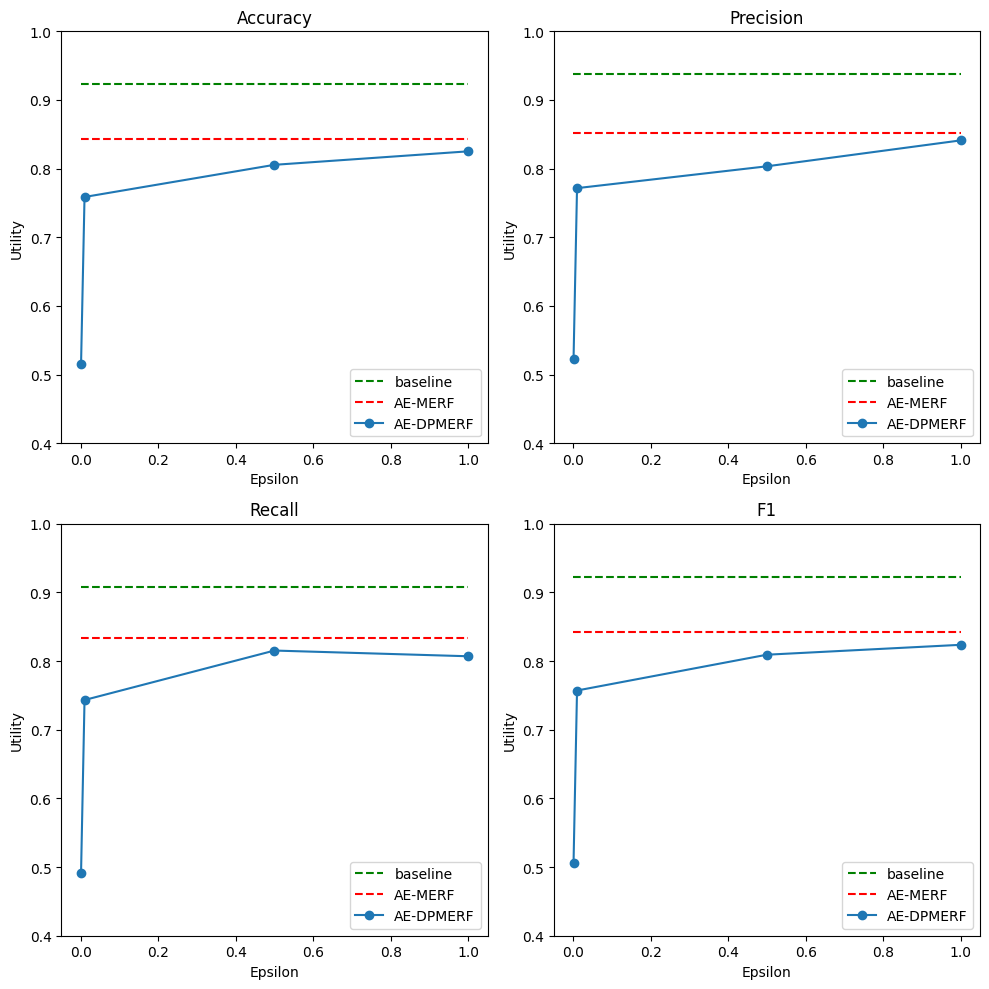
\includegraphics[scale=0.23]{results_aedpmerf.png}
        \caption{Results of AE-(DP)MERF with different privacy budgets (lower epsilon means higher privacy)}
        \label{fig:enter-label}
    \end{figure}
\end{frame}

\begin{frame}{(DP-)RTSGAN}
    \begin{figure}
        \centering
        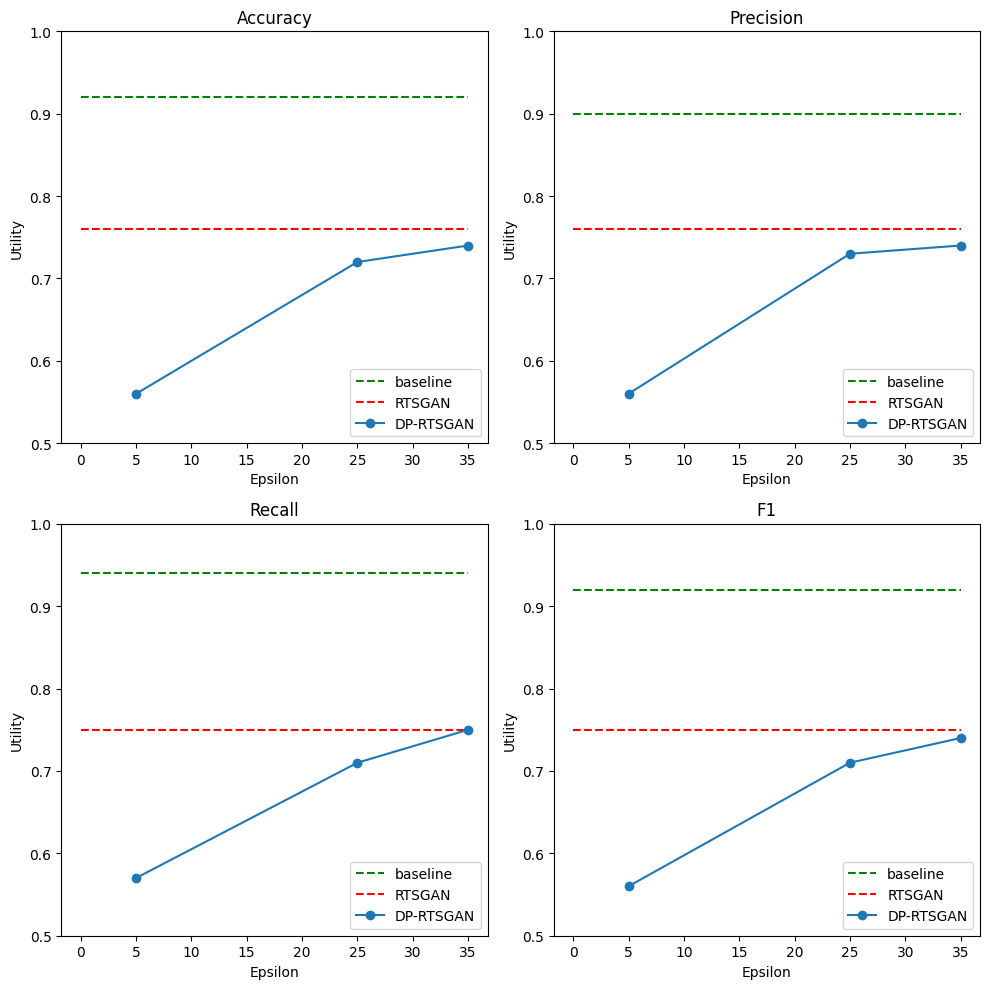
\includegraphics[scale=0.23]{restuls_dprtsgan.png}
        \caption{Results of (DP-)RTSGAN with different privacy budgets (lower epsilon means higher privacy)}
        \label{fig:enter-label}
    \end{figure}
\end{frame}

\begin{frame}{Conclusion}
    \begin{itemize}
        \item DPMERF performs best and is very efficient computationally.
        \item DPMERF can work in lower epsilon ranges, which translates to higher privacy guarantees.
        \item DP-RTSGAN gives worse generative performance and can only work with meaningless privacy budgets epsilon.
        \item Adding privacy does not impact the utility for anomaly detection too much until too much noise is added.
    \end{itemize}
\end{frame}

\begin{frame}{Contamination}
    We contaminate the train set that only consists of normal samples with 1\%, 2\%, 5\% anomalous samples (the percentage of heartbeat arrhythmias is estimated to be around max. 5\%).
\end{frame}

\begin{frame}{Contamination: AE-(DP)MERF}
    \begin{figure}
        \centering
        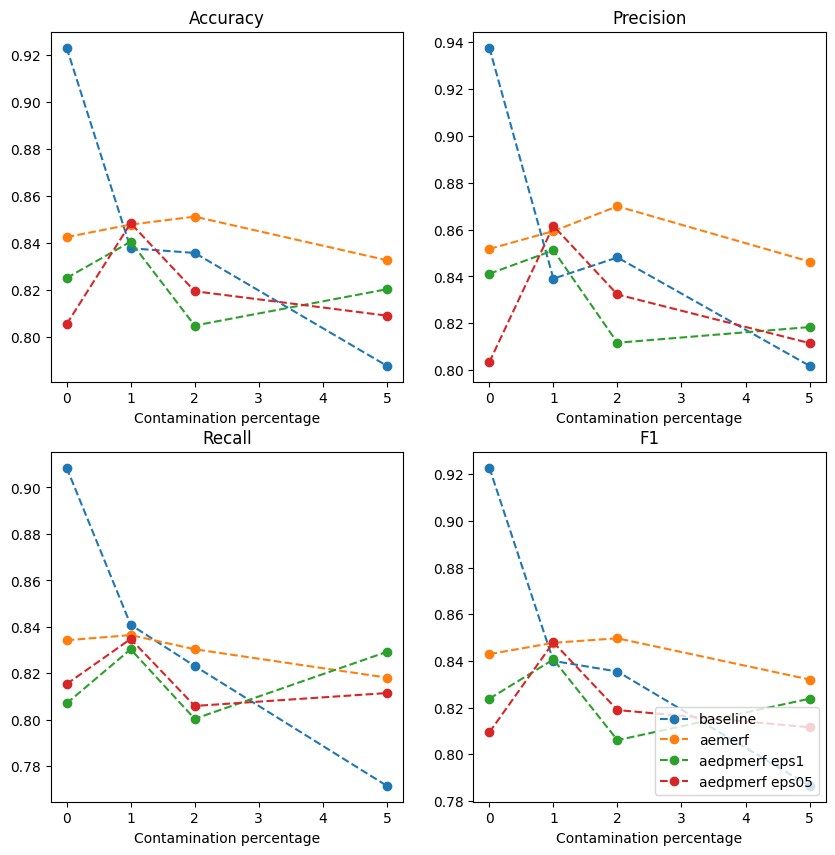
\includegraphics[scale=0.33]{results_aedpmerf_contam.png}
        \caption{Contaminated training set: AE-(DP)MERF}
        \label{fig:enter-label}
    \end{figure}
\end{frame}

